\renewcommand{\fpath}{C01-Body/Figures}
\chapter{Introduction}
\label{ch:introduction}

%%%%%%%%%%%%%%%%%%%%%%%%%%%%%%%%%%%%%%
%% Single Image

\begin{figure}[ht!]
	\centering
	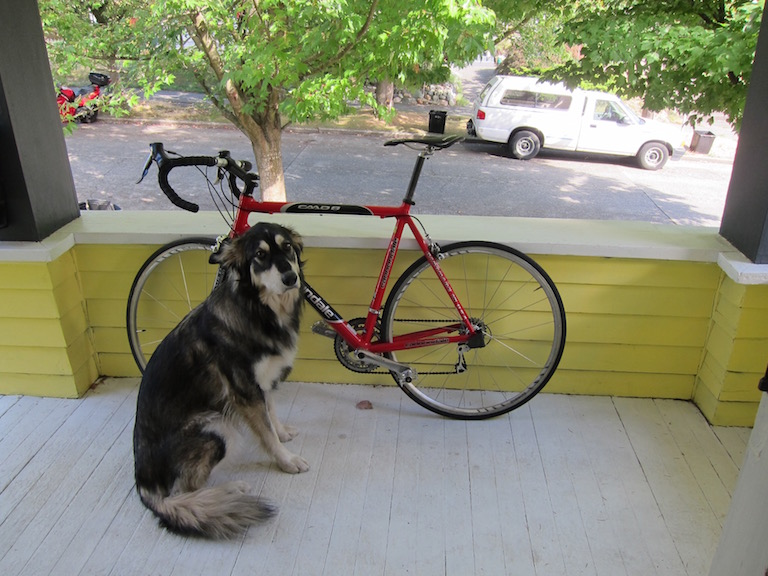
\includegraphics[width=0.46\textwidth]{\fpath/dog.jpg}
	\caption{An image of a dog.}%
	\label{fig:dog}
\end{figure}

% OR USING THE CUSTOM function
% (does exactly the same, simple removal of clutter)
% (simplification of code)
\singlefigure
{fig:dog}{dog.jpg}{0.46}{An image of a dog.}

%\singlefigure
%{<img_label>}{<img_name>}{<img_wdith>}{<img_caption>}

%%%%%%%%%%%%%%%%%%%%%%%%%%%%%%%%%%%%%%
%% 2 Images side-by-side
\begin{figure}[ht!]
	\begin{subfigure}[H]{0.46\textwidth}
		\centering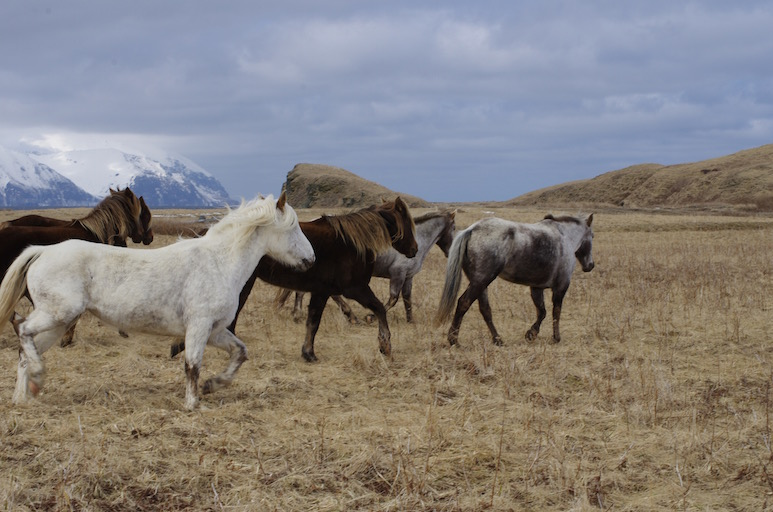
\includegraphics[width=\textwidth]{\fpath/horses.jpg}
		\caption{}%
		\label{fig:horses}
	\end{subfigure}
	\begin{subfigure}[H]{0.46\textwidth}
		\centering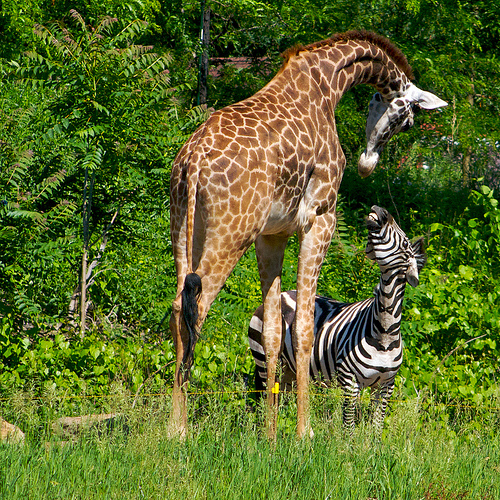
\includegraphics[width=\textwidth]{\fpath/giraffe.jpg}
		\caption{}%
		\label{fig:giraffe}
	\end{subfigure}
	\caption{(a) Horses image. (b) Giraffe image. Notes about both images, etc.}
	\label{fig:horses_and_giraffes}
\end{figure}

% OR USING THE CUSTOM function
% (does exactly the same, simple removal of clutter)
% (simplification of code)
\doublefigure{fig:horses_and_giraffes}%
{fig:horses}{horses.jpg}{0.46}{Horses image.}%
{fig:giraffe}{giraffe.jpg}{0.46}{Giraffe image.}
{Notes about both images, etc.}

%\doublefigure{<fullfigure_label>}
%{<img1_label>}{<img1_name>}{<img1_wdith>}{img1_caption}
%{<img2_label>}{<img2_name>}{<img2_wdith>}{img2_caption}
%{<both_img_caption>}
